\newpage
\section{Durchführung}

\subsection{Klassifizierung von Audiodateien durch ein Neuronales Netz}
Durch das neuronale Netz sollen digitale Audiodateien (Audiosamples) mit variabler Länge in fünf Merkmalsklassen klassifiziert werden. Dabei kann ein Datenpunkt, also ein Audiosample, mehreren Merkmalsklassen zugehörig sein. Dies wird als ``Multi-Label-Klassifizierung`` bezeichnet \cite{multilabel-classification}. Wird eine Audiodatei (Eingabevektor) zur Klassifizierung in das neuronale Netz eingegeben, erhält man als Ausgabe einen Ausgabevektor von fünf Werten zwischen 0.00 und 1.00, wobei jeder der fünf Werte  die Ähnlichkeit mit einer der fünf Merkmalsklassen repräsentiert (0.00 $\equiv$ keine Ähnlichkeit, 1.00 $\equiv$ Übereinstimmung). Die Merkmalsklassen werden wie folgt definiert:
    \begin{itemize}
        \item \textbf{bass:} Das Audiosample enthält Töne aus dem tiefen Frequenzspektrum
       	\item \textbf{pitched:} Das Audiosample enthält Töne aus dem hohen Frequenzspektrum
        \item \textbf{melodic:} Das Audiosample enthält melodische Elemente
        \item \textbf{rhythmic:} Das Audiosample enthält rhytmische Elemente
        \item \textbf{sustained:} Das Audiosample enthält ``flächige`` Elemente, also ``langgezogene`` Töne
    \end{itemize}

Dieses neuronale Netz wird mit selbst generierten Trainingsdaten trainiert und anschließend als fertiges Modell mittels dem STM32 proprietären Tool ``STM32Cube.AI`` in C-Code umgewandelt. Damit kann das Neuronale Netz im eigenen Code als normale C-Funktion verwendet werden, mit dem Eingabevektor (Audiodaten) als Funktionsparameter und dem Ausgabevektor (Klassifikationsergebnis) als Rückgabewert. \cite{stm32-cube-ai-documentation}

\begin{wrapfigure}{r}{0.4\textwidth}
    \centering
    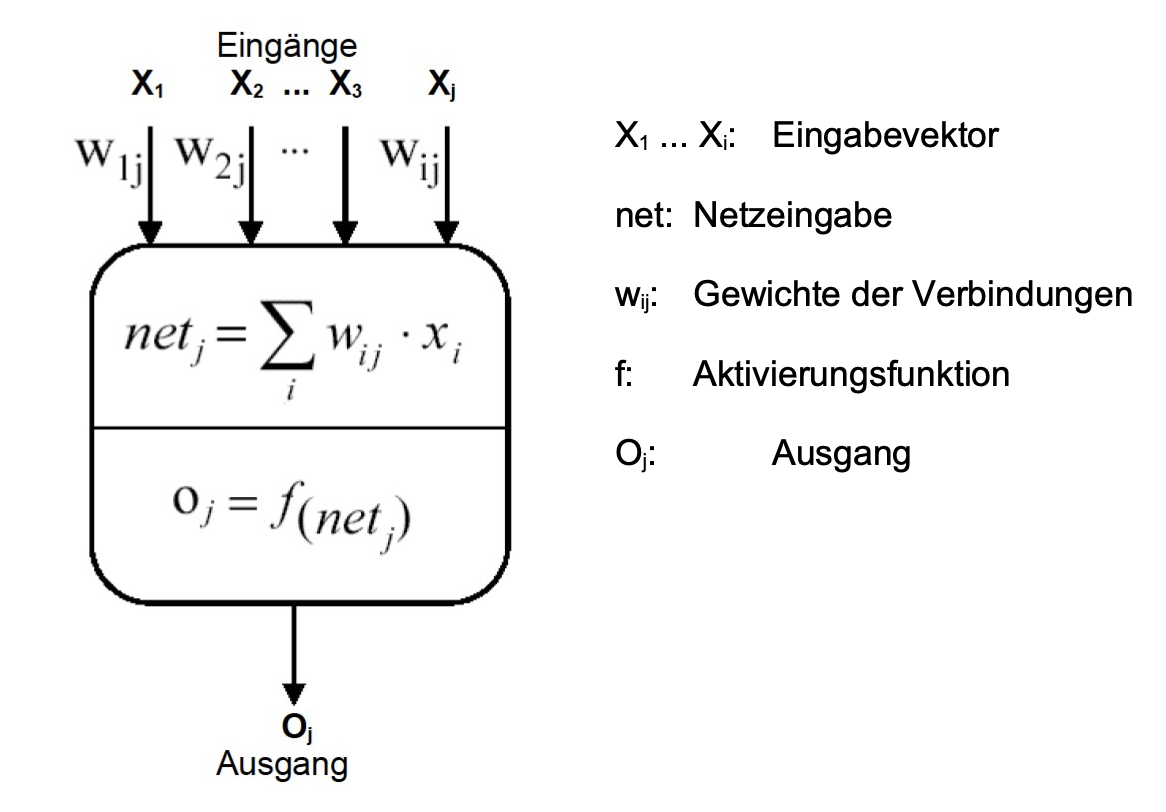
\includegraphics[width=0.4\textwidth]{images/08_durchfuehrung/neuron-aufbau.png}
    \caption{Aufbau des künstlichen Neurons. Quelle: Thieling, Lothar: “Neuronale Netze (Vorlesungsskript ML)”, Kapitel F, Seite 6.}
    \label{fig:img-aufbau-neuron}
\end{wrapfigure}

Die Umwandlung in C-Code ist mögich, da ein künstliches Neuron, wie in \textbf{\autoref{fig:img-aufbau-neuron}} dargestellt, aus aus mehreren Gewichten (\textit{W\textsubscript{x}}) in Form eines Vektors besteht, der mit dem Eingabevektor (\textit{X\textsubscript{n}}) des Neurons multipliziert wird. Beide Vektoren sind Fließkommazahlen. Anschließend werden diese Produkte aufaddiert und als Eingabewert einer mathematischen Funktion, der sog. ``Aktivierungsfunktion`` (\textit{f}) verwendet. Der Ausgabewert dieser Funktion ist die Ausgabe des Neurons. \cite{neural-network-basics}

Bei einem neuronalen Netz werden die Neuronen in Schichten hinterheinander angeordnet, die Neuronen der benachbarten Schichten werden vereinfacht gesagt miteinander verbunden, also die Eingabe des einen Neurons bildet eine der Eingaben des nachfolgenden Neurons. \cite{neural-network-basics}

Sowohl die Multiplikation von Vektoren, als auch die Berechnung von Funktionswerten ist in der Programmiersprache C problemlos möglich.

Der ressourcenintensive Teil des Umgangs mit neuronalen Netzen ist das Training, also der Anpassung der Gewichtswerte bis das Neuronale Netz akzeptable Ausgabewerte liefert \cite{neural-network-basics}. Bei diesem Prozess müssen vergleichsweise sehr viele Berechnungen durchgeführt werden. Aus diesem Grund wird das Neuronale Netz zuerst trainiert und erst dann als fertiges Modell in C-Code ungewandelt und auf dem STM32 Microcontroller betrieben. 
Dass das Neuronale Netz fortlaufend durch Benutzerinteraktion weiter trainiert wird, ist nicht vorgesehen.


\subsubsection{Ansatz für die Klassizierung von Audiodaten}
\label{sec:approach-audio-classification}
Die Audiosamples liegen als WAVE-Dateien (Dateiendung .wav) vor. Diese enthalten in der Regel pulsweitenmodulierte (PCM) Audiodaten \cite{wav-contains-pcm-data}. Da die Daten nicht komprimiert sind, gehören sie in der Audio- und Musikindustrie zu den gängigsten Dateiformaten \cite{wav-popular-file-format-music-industry}. Eine typische Samplerate für WAVE-Dateien beträgt 44,1 kHz, also 44.100 Samples pro Sekunde, wobei ein Sample in der WAVE-Datei ein quantisierter Amplitudenwert zu einem bestimmten Zeitpunkt ist \cite{wav-pcm-data}. Plottet man dies als Graph, könnte ein Audiosignal wie in \textbf{\autoref{fig:img-pcm-graph}} aussehen.


\begin{figure}[h!]
\centering
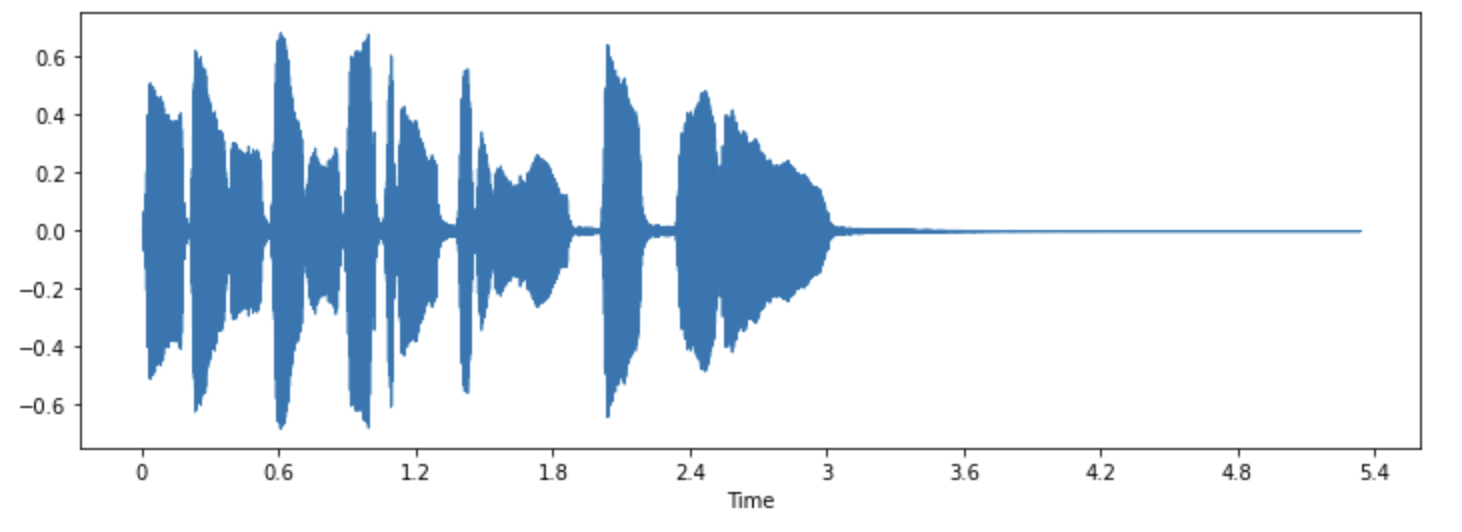
\includegraphics[width=0.6\textwidth]{images/08_durchfuehrung/waveform_plot.png}
\caption{Darstellung eines PCM Audiosignals, Quelle:  https://huggingface.co/learn/audio-course/chapter1/audio\_data TODO }
\label{fig:img-pcm-graph}
\end{figure}

Diese Daten direkt durch ein neuronales Netz klassifizieren zu lassen, ist aus verschiedenen Gründen wenig praktikabel. Die zwei Hauptgründe sind die Merkmalsextraktion und die Größe des Eingabevektors. Letzterer Punkt würde dazu führen, dass selbst bei einer geringeren Samplerate von 16 kHz der Eingabevektor 16.000 Werte umfasst. Ein Downsampling auf eine deutlich geringere Zahl, z.B. 1000, ist aufgrund des Shannon-Nyquist-Theorems nicht praktikabel, da dieses besagt, dass die Samplerate mindestens doppelt so hoch sein muss wie die höchste Frequenz \cite{nyquist}. Damit läge der klassifizierbare Frequenzbereich nur im Bereich von \textit{0 Hz} bis maximal \textit{1000 / 2 = 500 Hz}.

Deutlich geeigneter ist es, die Daten als Spektrogramm (Amplitude der verschiedenen Frequenzen eines Signals über die Zeit) wie in \textbf{\autoref{fig:img-spectrogram}} darzustellen und mit einem Convolutional Neural Network (CNN) zu klassifizieren. CNNs werden in erster Linie zur Klassifizierung von Bildern eingesetzt. Die wesentliche Idee ist, dass das neuronale Netz dann nicht nur klassifiziert, sondern auch die Bildvorverarbeitung und die Merkmalsextraktion übernimmt \cite{how-cnn-work}. Da die Audiodateien für das menschliche Gehör klassifiziert werden, sind Mel-Spektrogramme besonders geeignet. Sie basieren auf der Mel-Skala, die das menschliche Gehör nachahmt. Die Mel-Skala ist eine nichtlineare Skala der Frequenzen, die mehr Gewicht auf tiefere Frequenzen legt \cite{mel-spectrogram}.

\begin{figure}[h!]
\centering
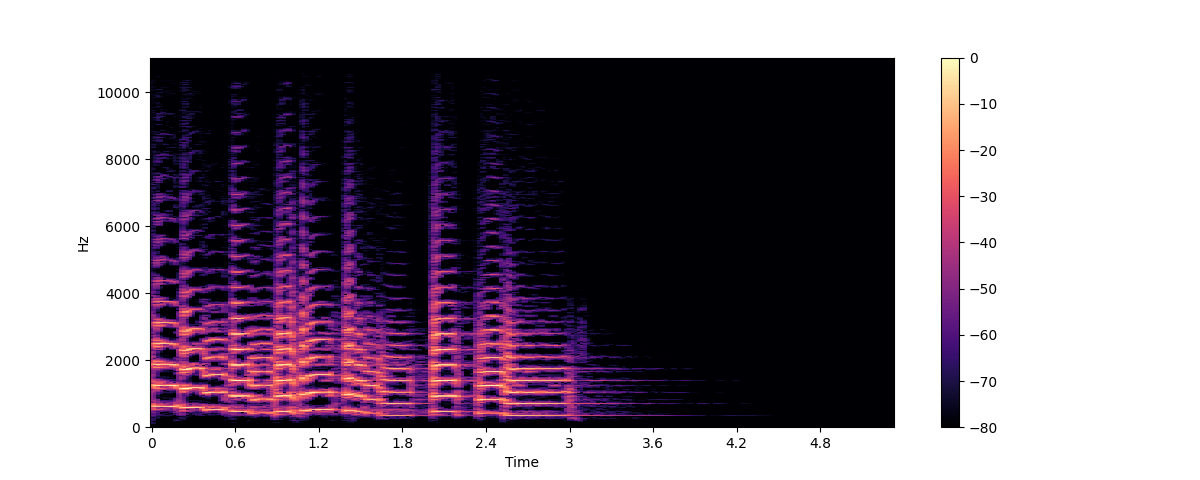
\includegraphics[width=0.75\textwidth]{images/08_durchfuehrung/spectrogram_plot.png}
\caption{Darstellung eines Audiosignals als Spektrogramm, Quelle:  https://huggingface.co/learn/audio-course/chapter1/audio\_data TODO }
\label{fig:img-spectrogram}
\end{figure}

Der limitierende Faktor beim Einsatz eines CNN auf einem Microcontroller sind die Hardwareressourcen, also in erster Linie Flash-Speicher und RAM.

Aufgrund der fehlenden Erfahrungswerte der Teammitglieder mit der möglichen Komplexität von neuronalen Netzen, die mit den Hardwareressourcen eines Microcontrollers betrieben werden können, wird sich auf ein Beispielprojekt von STMicroelectornics gestützt. Dieses heißt ``Acoustic Scene Classification`` \cite{stm-asc}\cite{stm-asc-2}. Kern ist die Klassifizierung von 30x32 px großen Mel-Spektrogrammen mit einem zwei Schichten CNN, die einen Eingabevektor von \textit{32 x 30 = 960} Werten ergeben. 

Sowohl die Dimensionierung der Spektrogramme, als auch die Topologie des Neuronalen Netzes, die Anzahl der Neuronen je Schicht und Elemente der Datenvorverarbeitung wurden aus diesem Projekt übernommen. Damit ist sicher gestellt, dass das Neuronale Netz am Ende nicht die Ressourcen des Microcontrollers übersteigt.

\subsubsection{Generieren der Eingabedaten}
\label{sec:input-data-generation}
Für das Training des neuronalen Netzes sind Trainingsdaten erforderlich. Diese bestehen aus Eingabedaten, die bereits mit den korrekten Klassifikationsergebnissen, also Labels, versehen sind. Um das Training des neuronalen Netzes während des Trainings einschätzen und nach Abschluss des Trainings validieren zu können, werden die Eingabedaten in drei Segmente aufgeteilt.

Da online keine kostenlosen und bereits mit den passenden Labels versehene Datensätze gefunden werden konnten, wurden eigene Daten generiert. Grundlage hierfür bildet eine private Audiosample-Bibliothek. Ein eigens entwickeltes Python-Skript ermöglicht es, Audiosamples auszuwählen, abzuspielen und zeiteffizient zu labeln.

Für jedes manuell gelabelte Audiosample wird eine eindeutige Identifikationsnummer (UID) generiert. Die zugehörigen Labels werden in einer CSV-Datei gespeichert. Ein Beispiel für einen solchen Datensatz zeigt \textbf{\autoref{tab:audiodaten}}. Außerdem wird eine Kopie des Audiosamples unter dem Namen der UID im Ausgabeordner des Skripts abgelegt. Diese Dateien werden später vom Jupyter-Notebook für das Training verwendet.

\begin{table}[h!]
\centering
\begin{tabular}{|m{2.8cm}|m{4.5cm}|m{0.8cm}|m{1.2cm}|m{1.5cm}|m{1.5cm}|m{1.3cm}|}
\hline
\textbf{UID} & \textbf{File} & \textbf{bass} & \textbf{pitched} & \textbf{sustained} & \textbf{rhythmic} & \textbf{melodic} \\ \hline
ecfad96b740844c3
9c96127279f22cf6 &  BD 606 Long MPC60 01.wav & 1 & 0 & 0 & 1 & 0 \\ \hline
\end{tabular}
\caption{Beispielhafter Datensatz eines Audiosamples}
\label{tab:audiodaten}
\end{table}

Bei der Auswahl der Audiosamples wurde darauf geachtet, dass die Daten annähernd gleich verteilt sind, um eine ausgewogene Trainingsbasis zu schaffen. Ein Ungleichgewicht in den Daten kann sich negativ auf das Training und die Klassifikationsergebnisse auswirken. Überrepräsentierte Merkmale könnten die Klassifikationsschwellenwerte beeinflussen, sodass die häufiger vorkommenden Klassen später bevorzugt erkannt werden. Wie in \textbf{\autoref{tab:img-class-spread-graph}} zu sehen, ist die Gleichverteilung jedoch zugegebenermaßen nur mäßig gelungen und hätte einen größeren Zeitaufwand erfordert.

\begin{figure}[h!]
\centering
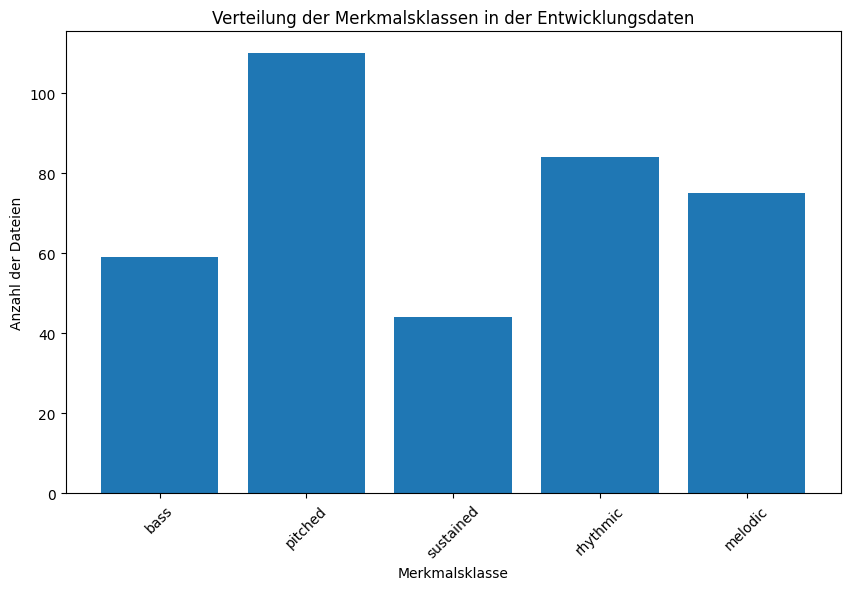
\includegraphics[width=0.75\textwidth]{images/08_durchfuehrung/class_spread_plot.png}
\caption{Repräsentation der verschiedenen Merkmalsklassen in den Entwicklungsdaten}
\label{fig:img-class-spread-graph}
\end{figure}

Zudem wurde sichergestellt, dass der Variationsbereich jeder Klasse möglichst umfassend abgedeckt ist. Dies umfasst sowohl reine Formen jeder Klasse – beispielsweise bei „pitched“ Audiosamples ausschließlich mit Tönen aus dem hohen Frequenzbereich – als auch Mischformen, die Merkmale mehrerer Klassen kombinieren.

Insgesamt wurden 207 Audiosamples unterschiedlicher Länge mit Labels versehen.

Insgesamt wu
TODO:

- wie viele Eingabe-Audiosamples

- wie viele Trainingsdatensätze

- Aufteilung der Daten (Grafik)

- Quellen

\subsubsection{Datenvorverarbeitung}

Für die Datenvorverarbeitung und das Training des neuronalen Netzes wird ein Jupyter-Notebook verwendet. Dieses ermöglicht eine Kombination aus formatiertem Text und Python-Code, was die Lesbarkeit und Nachvollziehbarkeit des Codes erleichtert.

Damit die gelabelten Daten für das Training des neuronalen Netzes verwendet werden können, müssen sie zunächst aufbereitet bzw. vorverarbeitet werden. Um die zu verarbeitenden Datenmengen sinnvoll zu verringern, wird zunächst die Samplerate aller Audiosamples auf 16 kHz reduziert.

Wie im Abschnitt \ref{sec:input-data-generation} erwähnt, liegen die Audiosamples als WAVE-Dateien unterschiedlicher Längen vor. Die in Abschnitt \ref{sec:approach-audio-classification} beschriebenen Dimensionen der durch das neuronale Netz klassifizierbaren Mel-Spektrogramme betragen 32x30 Pixel. Um bei unterschiedlich langen Audiosamples die zeitliche Abhängigkeit zu bewahren und auch bei längeren Audiosamples wichtige Informationen im Spektrogramm abzubilden, müssen die Audiosamples in Sektionen gleicher Länge unterteilt werden, wobei später aus jeder Sektion ein Spektrogramm erstellt wird. Diese Sektionen werden im Folgenden als „Audiosubsamples“ bezeichnet.

Ein Audiosubsample, also ein Mel-Spektrogramm, entspricht dabei 16.384 Frames, was bei einer Samplerate von 16 kHz etwas mehr als einer Sekunde entspricht. Analog zum Beispielprojekt „Acoustic Scene Classification“ \cite{stm-asc}\cite{stm-asc-2} werden die Audiosubsamples anschließend mittels eines „Sliding Window“ in 1024 Samples lange, um 512 Samples überlappende, Frames unterteilt. Diese Überlappung stellt sicher, dass Informationen zu den Anfangs- und Endzeitpunkten der Frames nicht durch das „Abschneiden“ verloren gehen. Die Aufteilung der Audiosamples in Audiosubsamples und Frames wird in \textbf{\autoref{fig:img-audiosubsamples-frames-overview} }visualisiert.

\begin{figure}[h!]
\centering
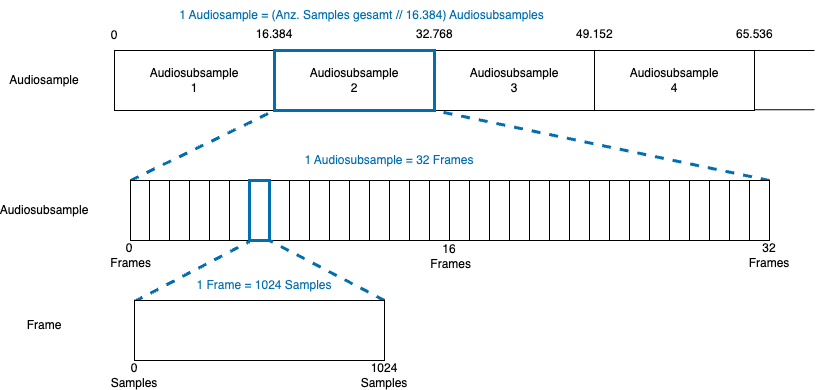
\includegraphics[width=0.8\textwidth]{images/08_durchfuehrung/audiosubsamples_frames_overview.png}
\caption{Darstellung der Unterteilung der Audiosamples in Audiosubsamples und Frames}
\label{fig:img-audiosubsamples-frames-overview}
\end{figure}

Das Sliding Window Prinzip, mit dem Audiosubsamples in überlappende Frames unterteilt werden, ist in \textbf{\autoref{fig:img-sliding-window}} dargestellt.

\begin{figure}[h!]
\centering
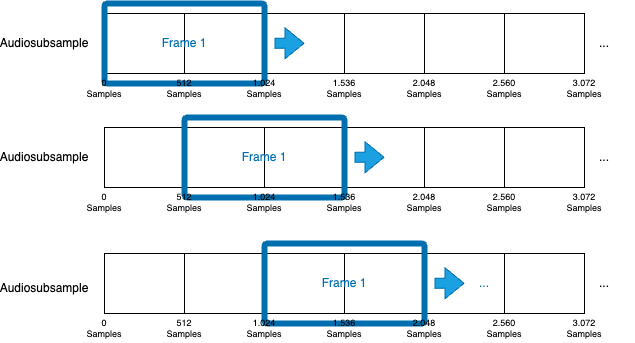
\includegraphics[width=0.7\textwidth]{images/08_durchfuehrung/sliding_window.png}
\caption{Darstellung des Sliding Window Prinzips}
\label{fig:img-sliding-window}
\end{figure}

Nun können die Mel-Spektrogramme erstellt werden. Eine Spalte des Spektrogramms wird dabei aus einem Frame berechnet. Setzt man die 32 in einem Audiosubsample enthaltenen Frames, also Spektrogramm-Spalten, zusammen, erhält man das 32x30 Pixel große Spektrogramm für ein Subsample.

Abschließend müssen die erhaltenen Daten standardisiert, also mittelwertfrei gemacht werden. Dies ist beim maschinellen Lernen üblich und sorgt dafür, dass das Modell schneller und effizienter konvergiert, indem es die Varianz in den Eingabedaten reduziert und eine gleichmäßige Verteilung der Werte gewährleistet. Damit diese Standardisierung später beim Einsatz des neuronalen Netzes auf dem Mikrocontroller nachgeahmt werden kann, werden die Werte des Scalers, der die standardisierten Werte berechnet, exportiert.


\subsubsection{Aufteilen der Eingabedaten in Trainings- Test und Validierungsdaten}

\subsubsection{Training des Neuronalen Netzes}

TODO:

- Topologie

- Trainignsparameter und warum (Adam (?), Learning Rate, no. epochs, etc.)

- erklären wann Training zu Ende

- accuracy bla graph

- confusion matrix

- model.h5

(und in Validierng einfach nur eigene samples eingeben und schauen bzw. hier drauf verweisen)




\subsubsection{Betrieb des Neuronalen Netzes auf dem STM32 Microcontroller}
TODO:

- wieder Datenvorverarbeitung

- Scaler

- Vorgehen Cube.AI (model.h5)

- Inference Zeit

- Verweis auf Validierungs-Kapitel



\begin{itemize}
    \item Implementierung der Komponenten:
    \begin{itemize}
        \item Ansätze/Methoden: Beschreibung der Ansätze und Methoden für jedes Teilprojekt
        \item Verwendete Komponenten: Detaillierte Beschreibung der verwendeten Komponenten
        \item Erkenntnisse während der Implementierung: Erfahrungen und Änderungen während der Implementierung und Begründung für Alternativen
    \end{itemize}
    \item Integration der Komponenten: Integration der Komponenten in das Gesamtsystem (aus zeitlichen Gründen nicht erfolgt)
\end{itemize}


\subsubsection{Downsampling für die Verarbeitung von Audio durch das Neuronalen Netzes}



\subsection{Audio Engine des Samplers}


Die Hauptfunktionalität eines Audiosamplers ist natürlich das Aufnehmen und Abspielen von Audiosamples. 

Der ausgesuchte PCM5102a Audio Codec bietet leider nur einen Ausgabestream, was eine Neubestellung eines Codecs mit In/Output Stream bedeuten würde, um auch die Aufnahme zu implementieren.

Angesichts des eh schon ambitionierten Featureumfangs und der damit verbundenen Zeitknappheit, wurde die also Aufnahmefunktion gekürzt, sodass der Prototyp zu einer reinen ``Sample-Playback`` Maschine wird. (TODO Verweis auf Lastenfall)


Das folgende Kapitel befasst sich mit der Implementierung und Ansteuerung der Audiowiedergabe über den Audio Codec.

Zunächst folgt eine Erläuterung des grundlegenden Signalfluss der Audioengine:

\subsubsection{Signalfluss der Audioengine}

Alle Audiosamples werden auf einer angeschlossen \textbf{SD Karte} persistent gespeichert. Diese werden dann immer stückweise mit dem \textbf{FATFS} Dateisystem, welches für eingebettete Systeme optimiert ist, in die Applikationslogik und somit den Audiopufferspeicher geladen. 

Von hier aus reicht die \textbf{DMA} den Buffer per \textbf{I2S} Protokoll an den \textbf{Audio Codec} weiter. 

Der Audio Codec wandelt die digitalen PCM Signale in eine analoges Signal mit Line-Level (TODO: Line Pegel elektrisch angeben).

\begin{figure}[h!]
	\centering
	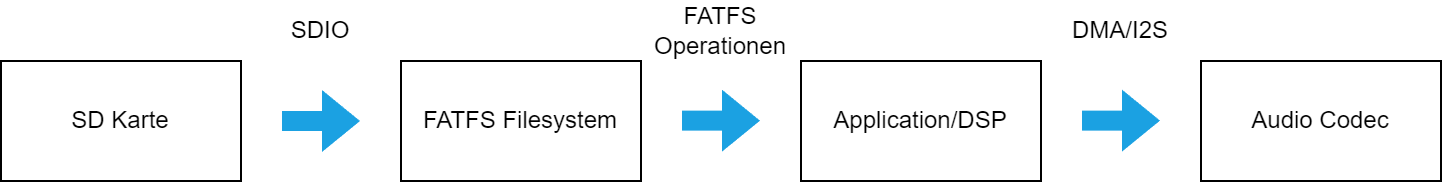
\includegraphics[width=0.6\textwidth]{images/08_durchfuehrung/audio/audio_signalflow.drawio.png}
	\caption{Digitaler Audio Signalfluss}
	\label{fig:audio_signalflow}
\end{figure}


\subsubsection{Latenzen}

TODO: TEST MIT MESSUNG IN TESTS (pulse an gpio geben, und audioausgang mit osci messen)

Echtzeitfähigkeit ist ein kritischer Aspekt bei elektronischen Audioinstrumenten. 
Eine niedrige Latenz ist entscheidend, um rhythmisch präzise und ``tight`` zu spielen, besonders wenn mehrere Instrumente miteinander synchronisiert werden müssen.

Die maximale Latenz, die ein menschlicher Profimusiker noch akzeptieren kann, liegt bei etwa 20ms. Diese Richtwert basiert auf der Wahrnehmungsgrenze, bei der Musiker und Live-Performern keine signifikante zeitliche Verzögerung zwischen dem Triggern eines Samples und dessen tatsächlichem Output am Ausgang spüren (https://www.highfidelity.com/backlog/how-much-latency-can-live-musicians-tolerate-da8e2ebe587a)

Um die Latenz auf ein Minimum zu reduzieren und sicherzustellen, dass elektronische Audioinstrumente reaktionsschnell und synchronisiert sind, können folgende Methoden angewendet werden:

\paragraph{Dimensionierung der Buffersize}\

Die erste Stellschraube ist die \textit{Buffersize}.
Das ist die Größe (in Bytes) des Audiobuffers.
Je kleiner der Audiobuffer, desto öfter pro Sekunde gibt die DMA dessen Inhalt an den Audio Codec weiter.

Das bringt jedoch auch Performanceeinbußen mit sich: Bei kleinen Audiobuffern hat die CPU, je nach Komplexität der durchzuführenden DSP-Operationen, möglicherweise nicht genug Zeit, um den gesamten Buffer zu verarbeiten.
Ein nur teils verarbeiteter Buffer kann hörbare Knackser und Störgeräusche am Ausgangssignal verursachen.

Hier gilt es also, die kleinstmögliche Buffersize zu ermitteln, ohne dass Störgeräusche auftreten.
Nach Experimentieren hat sich ein Wert von \textbf{128 Bytes} als adäquat herausgestellt.

\paragraph{Verwendung von Double Buffering}\

Double Buffering ermöglicht es, Daten in einem Pufferspeicher zu verarbeiten, während gleichzeitig ein anderer Puffer für die Eingabe oder Ausgabe verwendet wird. Dies reduziert Verzögerungen und ermöglicht eine nahtlose Datenverarbeitung, da der Prozessor nicht auf das Ende einer Übertragung oder Berechnung warten muss, bevor er fortfahren kann. (Quelle: https://www.eetimes.com/fundamentals-of-embedded-audio-part-3/)

\begin{figure}[H]
	\centering
	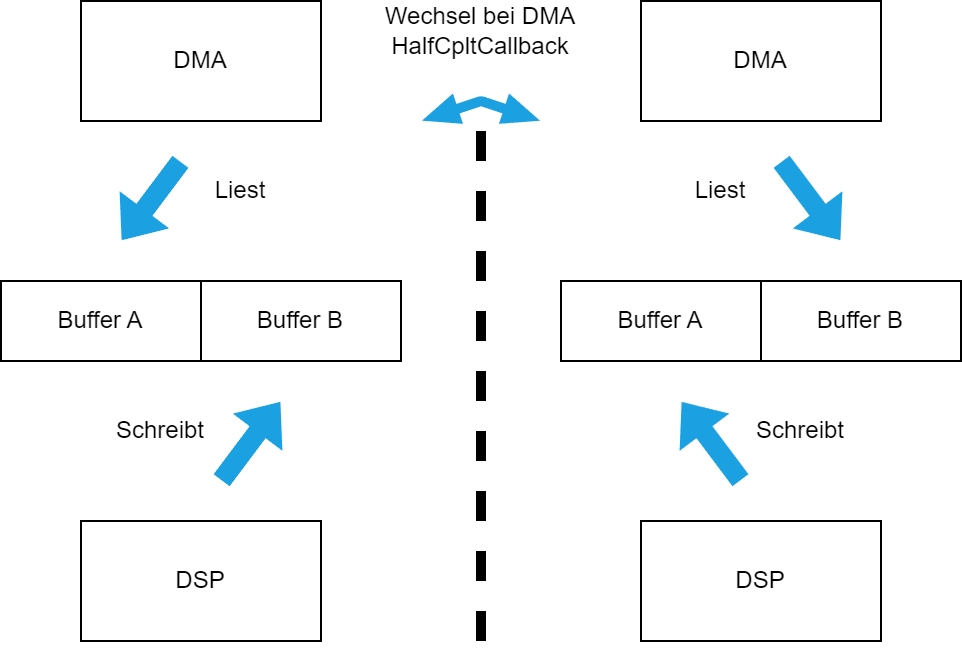
\includegraphics[width=0.6\textwidth]{images/08_durchfuehrung/audio/double_buffering.drawio.png}
	\caption{Double Buffering mit DMA und DSP}
	\label{fig:double_buffering}
\end{figure}


Bei I M A wird wird der Audiobuffer halbiert. 
Durch den Pointer \mintinline{c}|int16_t *outBufPtr| wird mit der DSP die Hälfte bearbeitet, die gerade nicht von der DMA übertragen wird.

In den Callback-Funktionen \mintinline{c}|HAL_I2S_TxHalfCpltCallback()| und \mintinline{c}|HAL_I2S_TxCpltCallback()| wird der Pointer auf die jeweilige Hälfte des Buffers, also auf (wie in  \textbf{\autoref{fig:double_buffering}} beschrieben:
\textbf{Buffer~A} und \textbf{Buffer~B}) gesetzt.


\inputminted[firstline=28, lastline=31]{c}{../../f401_sd_card_audio_codec_test/Core/Src/audio.c}

\inputminted[firstline=40, lastline=43]{c}{../../f401_sd_card_audio_codec_test/Core/Src/audio.c}


Diese Callbacks, werden automatisch aufgerufen, sobald die DMA die erste Hälfte, oder den gesamten Buffer übertragen hat. Sie eignen sich also sehr gut für die Setzung des Pointers.

Sobald das Flag \mintinline{c}|dma_dataReady == true| ist, wird die nächste Bufferhälfte von der SD Karte gelesen. 

\subsubsection{PCM5102a und I2S}

Ein sehr populäres Protokoll zur digitalen Audioübertragung ist I2S. Viele Codecs, so auch der PCM5102a unterstützen dieses Protokoll.

I2S (Inter-IC Sound) ist ein Standard für die digitale Übertragung von Audiodaten zwischen integrierten Schaltkreisen (ICs). Es wurde entwickelt, um die Kommunikation von digitalen Audiodaten zwischen verschiedenen Komponenten wie Mikrofonen, DACs (Digital-Analog-Wandler) und ADCs (Analog-Digital-Wandler) zu ermöglichen. 

TODO: PCM5102a Signale erklären (SCK, LCK, BCK, DIN)

Der PCM5102a erkennt komfortablerweise die eingehende Samplerate anhand der Bitclock.
Anders als bei vielen Audio Codecs ist keine zusätzliche Konfiguration des Chips über ein Kommunikationsprotokoll, wie I2C notwending.
Somit fallen auch keine Treiber für diesen Chip an.

- Der Einfachheit halber, festgelegte Samplerate und nur Stereo Samples! vllt eher zum DSP/Playback Part


\subsubsection{SD Karte}

Durch den sehr begrenzter RAM-Speicher des NUCLEO F401re Boards , ist es notwendig die Daten in Echtzeit von der SD-Karte zu streamen. Das setzt bei Stereo PCM Dateien, mit den gängigen Parametern, eine bestimmte Datenrate \( R \) voraus:

\begin{itemize}
	\item Abtastrate (Sampling Rate): 44.100 Hz (44,1 kHz)
	\item Bit-Tiefe: 16 Bit
	\item Kanäle: 2 (Stereo)
\end{itemize}


Die Datenrate \( R \) berechnet sich aus:

\[
R = \text{Sampling Rate} \times \text{Bit-Tiefe} \times \text{Anzahl der Kanäle}
\]



\[
R = 44{,}100 \, \text{Hz} \times 16 \, \text{bit} \times 2
\]

\[
R = 1{,}411{,}200 \, \text{bit/s} \approx 0.168 \, \text{MB/s}
\]


Theoretisch hätte eine Implementierung des FATFS-Dateisystems über SPI ausreichen müssen, um diese Datenraten zu bewältigen. 

Um die SDIO-Schnittstelle in das FATFS-Dateisystem zu integrieren, mussten zunächst Treiber entwickelt werden. Diese Treiber mappen die üblichen Dateioperationen wie \mintinline{c}|f_open()|, \mintinline{c}|f_read()| usw. über die SPI-Schnittstelle.


In der Praxis stellte sich jedoch heraus, dass der Audiobuffer nicht schnell genug gefüllt worden ist, was starke Knackser und Störgeräusche mit sich gebracht hat.

\begin{wrapfigure}{r}{0.3\textwidth} % Increase the width of the figure environment
	\vspace{-30pt + 0.02\textwidth}
	\hspace{0.02\textwidth} % Add horizontal space
	\fbox{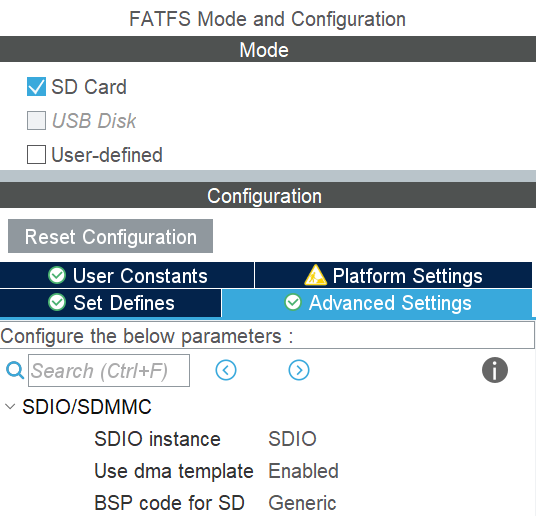
\includegraphics[width=0.28\textwidth]{images/08_durchfuehrung/audio/cubemx_sdio.png}}
	\caption{CubeMX FATFS SDIO Einbindung}
	\label{fig:cubemx_sdio}
\end{wrapfigure}

Dies erwies sich als äußerst vorteilhaft, da die SDIO-Implementierung zusammen mit FATFS direkt im Konfigurationstool von STM, \textbf{CubeMX}, ausgewählt werden kann. Die benötigten Treiber werden von CubeMX automatisch generiert und integrieren sich problemlos in das Dateisystem.

\subsubsection{Playback und Pitched Playback}


TODO Umsetzung im Code

CODE 

CODE 

CODE 

CODE 

CODE 

CODE 

CODE

CODE 




\subsection{Interface}\label{sec:interface}

Ein\textbf{ User Interface (UI)} in eingebetteten Systemen ermöglicht eine Interaktion zwischen Benutzer und Gerät.

Das \textbf{Interface} besteht aus \textbf{Encodern}, \textbf{Schiebepotentiometern}, einem \textbf{LCD-Display }und \textbf{Buttons}. Dessen Zusammenspiel ermöglicht dem Benutzer die nötige Kontrolle über den Sampler.


Im folgenden Kapitel wird Ihnen die Funktionalität, Implementierung, Ansteuerung, sowie das Zusammenspiel der Komponenten untereinander nähergebracht: 

\subsubsection{Encoder}
\textbf{Komponente \hyperlink{LF01_Link}{/LF01/}} \\

\textbf{Grundfunktionalität:} \\


Der \textbf{Encoder} dient der Navigation im Benutzer-Menü des Samplers. Er ermöglicht die Auswahl von Samples und das Scrollen durch die Sample-Liste, die auf dem LCD-Display angezeigt wird. Diese Liste zeigt die Namen der Samples an, die zuvor durch die Fader-Einstellungen bestimmt wurden. Der Cursor an der Seite zeigt die Aktuelle Position des Cursors an. Der Sample gilt als ausgewählt wen dessen Name unter der Liste erscheint.\\

\textbf{Umsetzung der Funktionalität:} \\

Die Auswahl von Samples sowie das Inkrementieren und Dekrementieren des Cursors, welcher sich im Struct des Filemanager befindet werden durch Interrupts unterstützt. Wenn der Encoder bewegt oder gedrückt wird, sendet er Signale an die MCU, die Interrupts auslösen.\\

Die Auswertung dieser Signale erfolgt dann in der Callback  \mintinline{c}|HAL_GPIO_EXTI_Callback(uint16_t GPIO_Pin)|. 

\begin{figure}[H]
	\centering
	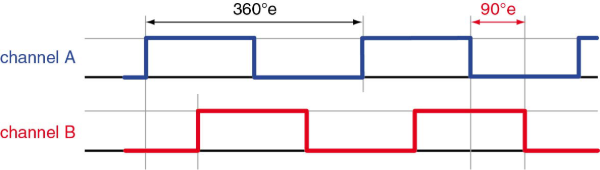
\includegraphics[width=0.8\textwidth]{images/08_durchfuehrung/interface/encoder.png}
	\caption{Phasenverschiebung A und B}
	\label{fig:phase_verschiebung}
\end{figure}

Wenn A und B beide High sind, wird die Cursor-Position welche in auf dem Display durch den Methodenaufruf \mintinline{c}|cursorUp(FileManager *fm)|
erhöht. Wenn  \textbf{\autoref{fig:phase_verschiebung}} A High und B Low ist, wird die Cursor-Position auf dem Display durch \mintinline{c}|cursorDown(FileManager *fm)| verringert. Wenn der Schalter gedrückt wird, wird die Datei durch \mintinline{c}|selectFile(FileManager *fm)| der Index des Files gespeichert. 

\newpage 
 \inputminted[firstline=68, lastline=74]{c}{../../f401_display_encoder_fader_test/Core/Src/filemanager.c}
 
  \inputminted[firstline=84, lastline=90]{c}{../../f401_display_encoder_fader_test/Core/Src/filemanager.c}
  
Anhand des Index des Files kann der Names des Files ermittelt werden.

	
\inputminted[firstline=159, lastline=161]{c}{../../f401_display_encoder_fader_test/Core/Src/filemanager.c}

\textbf{Problematik:}

Beim Drücken des Knopfes kann es in Systemen zu Mehrfachauslösungen kommen. Dies war auch beim Schalter des Encoders der Fall.

\textbf{Lösung:}

Um Mehrfachauslösungen zu verhindern, wurde ein Debouncing-Mechanismus implementiert. Dieser Mechanismus verwendet ein Flag \mintinline{c}|debounce| und einen Timer \mintinline{c}|tim3|, um wiederholte Auslösungen zu verhindern. Beim Drücken des Knopfes wird ein Interrupt ausgelöst, der eine Callback-Funktion \mintinline{c}|HAL_GPIO_EXTI_Callback(uint16_t GPIO_Pin)| aufruft. In dieser Callback-Funktion wird ein Flag gesetzt und ein Timer gestartet. Der Timer sorgt dafür, dass weitere Auslösungen innerhalb einer definierten Zeitspanne ignoriert werden, wodurch Mehrfachauslösungen effektiv verhindert werden.

Erst nach dem Ablauf des Timers war ist ein möglich den Knopf wieder zu betätigen.

\newpage
\subsubsection{Schiebenpotentiometer, ADC und DMA}
\textbf{Komponenten\hyperlink{LF02_Link}{/LF02/}} \\

\textbf{Grundfunktionalität:}\\

\textbf{Schiebepotentiometer} erfassen analoge Spannungen, die vom \textbf{Analog-Digital-Wandler (ADC)} in digitale Werte umgewandelt werden\textbf{\autoref{fig:conversion}}. Er nimmt in regelmäßigen Intervallen Proben des analogen Signals. Die Auflösung in 12 Bits 15 ADC Clock Cycles hat sich als am effizientesten herrausgestelt. ()\textbf{Wertebereich} 0-4096).

\begin{figure}[H]
	\centering
	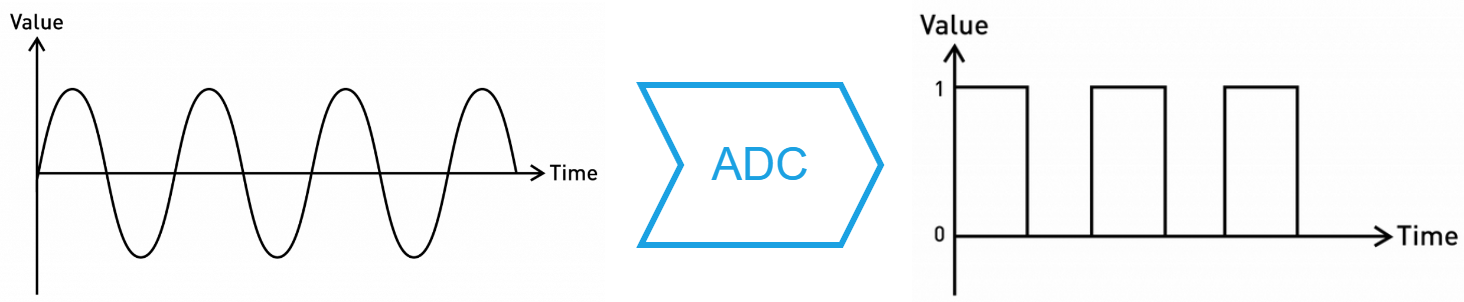
\includegraphics[width=1.0\textwidth]{images/08_durchfuehrung/interface/Conversion.drawio.png}
	\caption{ADC Conversion}
	\label{fig:conversion}
\end{figure}

Der \textbf{Direct Memory Access (DMA)-Controller} übernimmt anschließend die direkte Übertragung dieser digitalen Werte in den Speicher, konkret in  \mintinline{c}|adcBuffer[NUM_CHANNELS]|.

\begin{figure}[H]
\centering
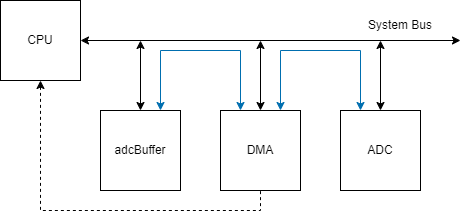
\includegraphics[width=0.8\textwidth]{images/08_durchfuehrung/interface/DMA_ADC_MEM.drawio.png}
\caption{DMA ADC FADER Bus System}
\label{fig:DMA_ADC_FADER}
\end{figure}

Der Direct Memory Access (DMA)-Controller ermöglicht die direkte Datenübertragung zwischen Speicher und Peripheriegeräten, wodurch die Prozessorbelastung reduziert wird. Analoge-Digital-Wandler (ADCs) sorgen für die schnelle Digitalisierung analoger Signale, was eine präzise Verarbeitung der Messdaten ermöglicht. Potentiometer bieten die Möglichkeit zur benutzerfreundlichen Anpassung von Spannungswerten. Das Bussystem sorgt für eine effiziente Kommunikation zwischen den verschiedenen Komponenten und gewährleistet eine konsistente und zuverlässige Datenverarbeitung. \textbf{\autoref{fig:DMA_ADC_FADER}} \\

\newpage
\textbf{Problematik:}

\textbf{No.1}

Bei der Implementierung der DMA traten Probleme auf, die dazu führten, dass der Bildschirm einfrohr und das Bedienen der Interfaces unmöglich wurde. Das Problem entstand, weil die DMA fortlaufend Daten übertrug und die CPU dadurch vollständig beansprucht wurde, um die Daten, die von der DMA übertragen wurden, zu verarbeiten. Dies führte zu einer Überlastung der CPU, da sie gezwungen war, sich auf die Verarbeitung der von der DMA bereitgestellten Daten zu konzentrieren, anstatt andere Aufgaben zu bewältigen. Infolgedessen konnten keine weiteren Systeminteraktionen durchgeführt werden, da die CPU keine Ressourcen mehr für andere Aufgaben zur Verfügung hatte.

\textbf{No.2}

Die Auswertung und Verarbeitung der Signale erfolgt in der \mintinline{c}| HAL_ADC_ConvCpltCallback(ADC_HandleTypeDef* hadc)|.

Im laufe der Implementation des ADC könnte man Schwankungen an den Ausgangssignalen des ADCs festellen, was die Genaugigkeit der Potentiometer einstellung beeinflüsste. 

\textbf{Lösung No.1:}

Um das Problem zu beheben, wurde ein \textbf{Timer} \mintinline{c}|tim5| implementiert, der die DMA-Übertragung steuert. Der Timer sorgt dafür, dass die DMA in regelmäßigen Intervallen gestartet und gestoppt wird. Diese Maßnahme ermöglicht es der CPU, sich ausreichend um andere Aufgaben zu kümmern, indem sie nicht kontinuierlich mit der Datenverarbeitung durch die DMA beschäftigt ist. Der Einsatz des Timers verhindert, dass die DMA die CPU überlastet und gewährleistet eine ausgewogene Nutzung der Systemressourcen. \\

\textbf{Lösung No.2:}

Diese Schwankungen würden behoben in dem man ein Glättung der Werte eingeführt hat.

Zunächst werden des \mintinline{c}|adcBuffer[i]| in \mintinline{c}|smoothValue[i]| aufeinander addiert. Dann wird derren Durchschnittswerte berechnet. Die geglätteten Werte werden für alle Kanäle des ADC berechnet. 

\textcolor{red}{TODO: Code Verschieben}

 \inputminted[firstline=121, lastline=135]{c}{../../f401_display_encoder_fader_test/Core/Src/interface.c}

Diese Glättung sorgt dafür, dass die Messwerte stabiler und weniger anfällig für zufällige Schwankungen sind. Anschließend werden die Durchschnittswerte ermittelt. Diese Durchschnittswerte dienen zwei Zwecken: Einerseits werden sie zur Anzeige auf dem Bildschirm verwendet  \mintinline{c}|currentClassPercentADC[]|
, andererseits sind sie für Vergleichsoperationen innerhalb des Sortieralgorithmus von Bedeutung  \mintinline{c}|fm.fader_Class[]|.
 Schließlich wird ein Zeichenarray \mintinline{c}|faderProzent[0]| initialisiert, das später auf dem Display angezeigt wird. 
 
Eine andere möglichkeit des Spannungs inkonsitenz könnte mit Kondensatoren umgesetzt werden was jedoch nicht umgesetzt würde aus zeitlichen Gründen.

\newpage
\subsubsection{Display, SD1306 Treiber und I2C}

\textbf{I2C} \\

\textbf{I2C} (Inter-Integrated Circuit) ist ein Kommunikationsprotokoll, das über zwei Leitungen arbeitet: \textbf{SDA} (Serial Data Line) und \textbf{SCL} (Serial Clock Line). Es verwendet eine Master-Slave-Architektur, bei der der Master die Kommunikation steuert und die Slaves Daten empfangen oder senden. Die Datenübertragung erfolgt in Byte-Paketen, wobei der Master eine Start-Bedingung sendet, gefolgt von der Adresse des Slaves und den Daten. Nach dem Empfang eines Datenbytes sendet der Slave ein Bestätigungsbit (ACK). Die Kommunikation endet mit einer Stop-Bedingung \textbf{\autoref{fig:I2C}}. \\

\textbf{Vorteile}\\

\begin{itemize}
	\item \textbf{Einfache Verkabelung}: Es werden nur zwei Leitungen für die Kommunikation benötigt, was den Verkabelungsaufwand erheblich reduziert.
	\item \textbf{Geringe Hardware-Kosten}: Die Implementierung von I2C ist kostengünstig und benötigt wenig zusätzliche Hardware, da die Logik für das Protokoll minimal ist.
	\item \textbf{Fehlererkennung}: \textbf{I2C} bietet einfache Methoden zur Fehlererkennung, wie das Bestätigungsbit (ACK), um sicherzustellen, dass Daten erfolgreich übertragen wurden.
	\item \textbf{Unterstützung von Standard-Bibliotheken}: Viele Mikrocontroller und Entwicklungsplattformen bieten Standard-Bibliotheken für \textbf{I2C}, was die Implementierung und Fehlerbehebung erleichtert.
\end{itemize}

\begin{figure}[H]
	\centering
	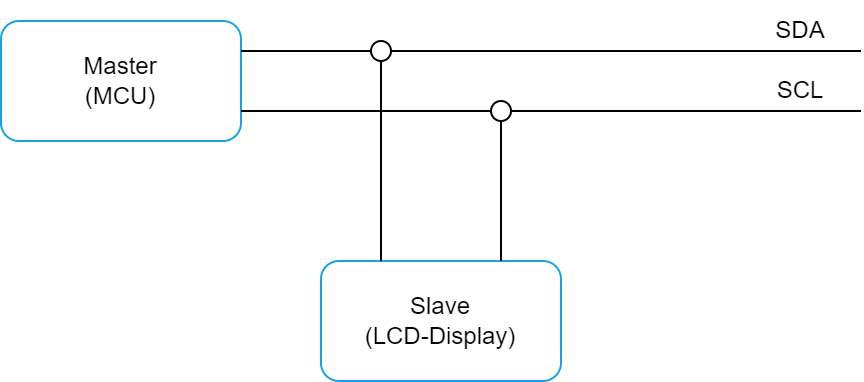
\includegraphics[width=0.8\textwidth]{images/08_durchfuehrung/interface/I2C.drawio.png}
	\caption{I2C Kommunikation}
	\label{fig:I2C}
\end{figure}

\newpage	
\textbf{Display} \\	


Das Display ist die zentrale Komponente des Interfaces, da es visuelles Feedback auf die Benutzerinteraktionen bietet. Die Kommunikation zwischen dem Nucleo F401RE-Mikrocontroller und dem Display erfolgt über das I2C-Protokoll. Der Mikrocontroller übernimmt dabei die Rolle des Masters, der den Bus steuert, während das Display als Slave agiert.

Die Ansteuerung des Displays erfolgt über den SD1306-Treiber, der als Schnittstelle zwischen dem Mikrocontroller Nucleo F401RE und dem LCD-Display fungiert. Der Treiber nutzt das I2C-Protokoll, um Befehle und Daten effizient zu übermitteln. Er sendet die erforderlichen Befehle an das Display und übernimmt die Kommunikation gemäß den I2C-Spezifikationen. Bei Bedarf kann die Initialisierungssequenz des Treibers angepasst werden, um auch SH1103-kompatible Bildschirme zu unterstützen \textbf{\autoref{fig:Display SD1306 I2C}}.

Zusammenfassend ermöglicht der SD1306-Treiber die vollständige Integration des Displays in das System, indem er die I2C-Kommunikation zwischen Mikrocontroller und Display umsetzt. \\ 


\begin{figure}[H]
	\centering
	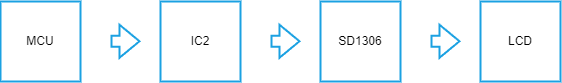
\includegraphics[width=1.0\textwidth]{images/08_durchfuehrung/interface/Display SD1306 Treiber I2C.drawio}
	\caption{Display SD1306 I2C Kommunikation}
	\label{fig:Display SD1306 I2C}
\end{figure}

Die beiden Hauptfunktionen zur Darstellung auf dem OLED-Bildschirm sind:

 \mintinline{c}|void  displayStrings(I2C_HandleTypeDef *hi2c1, char** strings, uint8_t numStrings, uint8_t cursor_index)|
 
 \mintinline{c}|void renderSelectedFile(I2C_HandleTypeDef *hi2c1, const char *filename)| bzw. 
 
 \mintinline{c}|drawFaderProzent| ähnliche funktionsweiße wie  \mintinline{c}|renderSelectedFile|. 


In der Funktion \mintinline{c}|displayStrings| werden die `ssd1306`-Funktionen verwendet, um die Strings auf dem LCD-Display darzustellen. Die Funktion \mintinline{c}|ssd1306_SetCursor| legt die Position für die Anzeige fest, und \mintinline{c}|ssd1306_WriteString| wird verwendet, um die Strings auf dem Display auszugeben. Bei der Anzeige des ausgewählten Strings wird zusätzlich ein Cursor-Symbol integriert.

In der Funktion \mintinline{c}|renderSelectedFile| wie bei \mintinline{c}|displayStrings| `ssd1306`-Funktionen verwendet, um den Namen der ausgewählten Datei auf dem OLED-Display darzustellen. Die Funktion \mintinline{c}|ssd1306_DrawPixel| wird verwendet, um den Bereich für die Dateianzeige zu löschen. Anschließend legt \mintinline{c}|ssd1306_SetCursor| die Position für die Textausgabe fest, und \mintinline{c}|ssd1306_WriteString| gibt den Namen der ausgewählten Datei auf dem Display aus. \\

\textbf{Problematik:} \\

Der ursprünglich verwendete SD1306-Treiber war nicht mit dem Display kompatibel. Der Fehler wurde durch die ungeeignete Initialisierungssequenz für das Display verursacht, was zu einer fehlerhaften Darstellung der Daten auf dem Bildschirm führte.

\textbf{Lösung:} \\

Die Anpassung der Definitionskonstanten, die als Befehle über I2C an das Display gesendet werden, sowie die Änderung der Schleifenbedingung in der Methode \mintinline{c}|ssd1306_UpdateScreen(I2C_HandleTypeDef *hi2c)| von einer Länge von 8 auf 16 haben das Problem behoben.
\newpage


\subsubsection{Dateisystem} 
\vspace{1em}

Das Dateisystem fungiert als zentrale Schnittstelle zwischen der Audio-Wiedergabe, dem neuronalen Netzwerk zur Klassifizierung und der Benutzeroberfläche. Es organisiert und verwaltet die Audiodateien, die vom neuronalen Netzwerk analysiert und klassifiziert werden. Nach der Klassifizierung speichert das Dateisystem die Ergebnisse und gewährleistet, dass nur relevante und korrekt kategorisierte Dateien im Interface angezeigt werden. Das Dateisystem besteht aus zwei Hauptstrukturen: File und FileManager welche Ihnen im folgenden nähr gebracht werden.

\vspace{1em}
\textbf{File}
\vspace{1em}

Die \boldinline{File}-Struktur repräsentiert einzelne Audiodateien im System. Sie enthält den Dateinamen, der sowohl für das Abspielen der Audiodatei als auch für die Anzeige in einer Liste von Samples verwendet wird. Zusätzlich speichert die Struktur Klassifizierungsdaten, die vom neuronalen Netzwerk bereitgestellt werden.


 \inputminted[firstline=37, lastline=41]{c}{../../f401_display_encoder_fader_test/Core/Inc/filemanager.h}
 
\vspace{1em}
\textbf{FileManager}
\vspace{1em}

Die \boldinline{FileManager}-Struktur repräsentiert das Dateisystem selbst. Sie ist verantwortlich für die Verwaltung und Speicherung von Dateien und umfasst wesentliche Elemente, die für die Visualisierung der Dateien auf dem LCD-Display erforderlich sind.
 
 \inputminted[firstline=49, lastline=58]{c}{../../f401_display_encoder_fader_test/Core/Inc/filemanager.h}
 
\vspace{1em} 
\textbf{Problematik:} \\



Das Schreiben der \boldinline{FileManager}-Struktur auf die SD-Karte war zunächst nicht möglich und konnte aus zeitlichen Gründen nicht behoben werden.



